\section{Breakdown}

\subsection{Rationale}

	The primary goal of Aim 3 will be to integrate the on-board micro-controller with the neural network developed in the Spring of 2022 by the computer science and engineering capstone team after it is trained on real anatomical footage. Their system utilizes a trained neural network to identify and trace the anatomical features of the airway from video records. The outputs of the identifier are boxes which encapsulate the feature, as well as a confidence interval value which relays how likely it is that the feature was identified correctly.

	The automation component of the device is wholly dependent on the system discussed here. It will most likely be implemented on board the device, but depending on its weight and specifications, it may be run on a separate unit, with a more complex communication system. Either way, the device will be capable of this feature with the addition of the camera to the end effector.
	
	Figure \ref{fig:cseproject_demo} shows a demonstration of the CSE team's newtork in progress. The results among all test were relatively similar, with some difficulty noticed as the camera approached the airway. That said, with more training the network should be able to overcome this issue. The footage referenced is currently held by the Wexner Medical Center under a XXX disclosure agreement, and will be released to this project for the express purpose of training the network.
	
	\begin{figure}[ht]
		\centering
		\includegraphics[scale=0.85]{cseproject_demo}
		\caption{Anatomy Identification Network on Human Mannequin}
		\label{fig:cseproject_demo}
	\end{figure}

\subsection{Approach}

	\subsubsection{Timeline}
		During the 2022 Spring semester, the BME department at the OSU commisioned a CSE department capstone project with the intent to develop a functional AI system. This network can be used to identify the anatomical features of the human mouth and airway. For the purpose of the project, the network was limited to identification of features on a mannequin, and the videos taken were processed and put through the network after they were taken. That said, the network developed was capable of identifying the uvula, epiglottis and vocal chords as shown in Figure \ref{fig:cseproject_demo}.
		
		To expand off of this project, three main tasks will be completed. First, the network will be retrained on the real-anatomy data set already collected by the Wexner Medical Center. This process will most likely be given about $40\%$ of the total project time, i.e. $5[months]$ in a year-long project.
		
		The network will then be integrated with the main controller hardware. This will most likely involve a communication system between the external network and the controller being programmed on for Aim 1 and the camera system. It is currently unclear how exactly this will be implemented, but time will be set aside specifically to problem solve this requirement. This process will also be given approximately $40\%$ of the total project time. It should be noted that Specific Aim 1 need not be completed for this process to be completed. As long as it can be proven that the hardware is able to read and utilize the output of the controller (even if that is simply outputting results to the screen), the test will be considered complete.
		
		The final test will consist of verifying that the identification software can be utilized in real time using the on-board camera. These tests will likely require the use of the mannequin, but will eventually be demonstrated on cadaver subjects as well (although the cadaver tests are unlikely to occur in this time frame). Again, these tests have no dependency on Aim 1 or 2 since the only system being verified is the identification system. This portion of the project will be given the remaining $20\%$ of the project timeline (around $2[months]$).

		The completed timeline, as well as those constructed for Aim 1 and 2, is shown in Figure \ref{fig:full_timeline}.
		
	\subsubsection{Network Testing and Integration}
		The neural network referenced here is largely sitting in a completed state. It is currently trained on a set of human mannequin example videos and performs to a high degree of accuracy. Once access is granted for the human intubation procedure videos housed on the Ohio State University Wexner Medical Center computer system, the network can be retrained for real human anatomy. The work done by the CSE department capstone team will be used to streamline this process, as they setup the neural network layers efficiently and were able to identify the anatomical features from human mannequin footage. The same network can thus be used for the real system.

		Once the network is trained, a communication system between the on-board micro-controller and the NN will be developed. The current plan is to evaluate the run-time needs of the neural network and quantify whether it can be run from within the housing module, or if it should be run externally and communicate via a wired connection. It should be noted that the control system from Aim 1 does not need to be finished to test this communication system. As long as the outputs from the network match the inputs to the controller, they can be developed in parallel. This means that at the beginning of both processes, the communication point will be defined thoroughly to alleviate any difficulties down the road.
	
	\subsubsection{Experimental Process}

\subsection{Risks and Alternatives}

	The largest risk in the development of the neural network is defining the level of confidence which the controller will allow before deciding a motion is safe. In other words, how low of a confidence is acceptable before the controller refuses to move in that direction. Setting this value too low factors in an obvious level of risk to the patient, as the device may navigate towards incorrectly identified features. Setting this setting too high may put the device at risk of stalling, i.e. reaching a point where no features are identifiable and not being able to make a decision. Ideally, a fail-safe will be implemented to account for this but it is also important to remember that the device as a whole is being designed with the intent that the practitioner is never absent from the procedure. They are required to watch the approach of the robot into the airway, and in these rare instances they would easily be able to manually override the neural network and move the robot in the proper direction.